\chapter{Background Suppression}\label{sec:background-suppression}

This chapter explains the procedure of suppressing various kinds of backgrounds by using MVA classifier outputs. More information about the MVA training, feature importance and hyper-parameter optimization for each MVA step in this chapter can be found in Appendix \ref{sec:mva-control-plots}.

\section{Resonant Background}
\label{sec:res_bkg}

In the analysis we study decays with kaons in the final state. This means that standard procedures in $b \to u$ analyses in order to suppress $b \to c$ backgrounds, such as $K$-veto, are not possible. As a consequence, our final sample consists of combinations of $K$ pairs coming also from $b \to c$  sources, such as $D^0 \to K^+ K^-$. Such candidates usually have resonance-like properties in the two-kaon invariant mass spectrum. Figure \ref{fig:res_bkg} shows this invariant mass spectrum of two kaons, $m_{KK}$, where obvious resonant structures are present from sources like
\begin{itemize}
	\item $\phi \to K^+K^-$ (sharp peak at $\sim1.019\e{GeV}/c^2$),
	\item $D^0 \to K^+K^-$ (sharp peak at $\sim 1.864\e{GeV}/c^2$),
	\item $D^0 \to K^+ \pi^-$ (wide, shifted peak, due to kaon miss-identification).
\end{itemize}

In order to suppress these resonant backgrounds, while studying signal or control decays, we define two regions
\begin{itemize}
	\item signal region:\\$\vert m_{KK} - m_{\phi} \vert > \Delta_\phi$, $\vert m_{KK} - m_{D^0} \vert > \Delta_{D^0}$, $\vert m_{K\pi} - m_{D^0} \vert > \Delta_{D^0}$,
	\item control region:\\$\vert m_{KK} - m_{D^0} \vert \leq \Delta_{D^0}$, $\vert m_{K\pi} - m_{D^0} \vert > \Delta_{D^0}$,
\end{itemize}

where $m_{KK}$ is the $KK$ invariant mass and $m_{K\pi}$ is the invariant mass of $KK$ candidates, where the kaon with the same charge as the $B$ meson was given the mass of the $\pi^0$. $m_\phi \approx 1.019\e{GeV}/c^2$ and $m_{D^0} \approx 1.864\e{GeV}/c^2$ are nominal masses of the $\phi$ and $D^0$ mesons, and $\Delta_\phi \approx 8\E{-3}\e{GeV}/c^2$ and $\Delta_{D^0} \approx 1.5\E{-2}\e{GeV}/c^2$ are the widths around the nominal mass values for the $\phi$ and $D^0$ meson, respectively. By selecting the signal or control region, we are able to efficiently isolate the desired subset. Table \ref{tab:cut_eff} shows the subsample efficiency after selecting either of the regions.

\begin{table}[H]
	\centering
	\begin{tabular}{l|c|c|c}
		& $\epsilon$(Signal cand.)& $\epsilon$(Control cand.) & $\epsilon$($\phi$ resonance cand.)\\
		\toprule
		Signal-specific & $95.4\%$ & $4.0\%$ & $13.6\%$ \\
		Control-specific & $1.9\%$ & $96.0\%$ & $0.0\%$ \\
		\bottomrule
	\end{tabular}
	\caption{Efficiencies after selecting the signal or control region}
	\label{tab:cut_eff}
\end{table}


\begin{figure}[H]
	\centering
	\captionsetup{width=0.8\linewidth}
	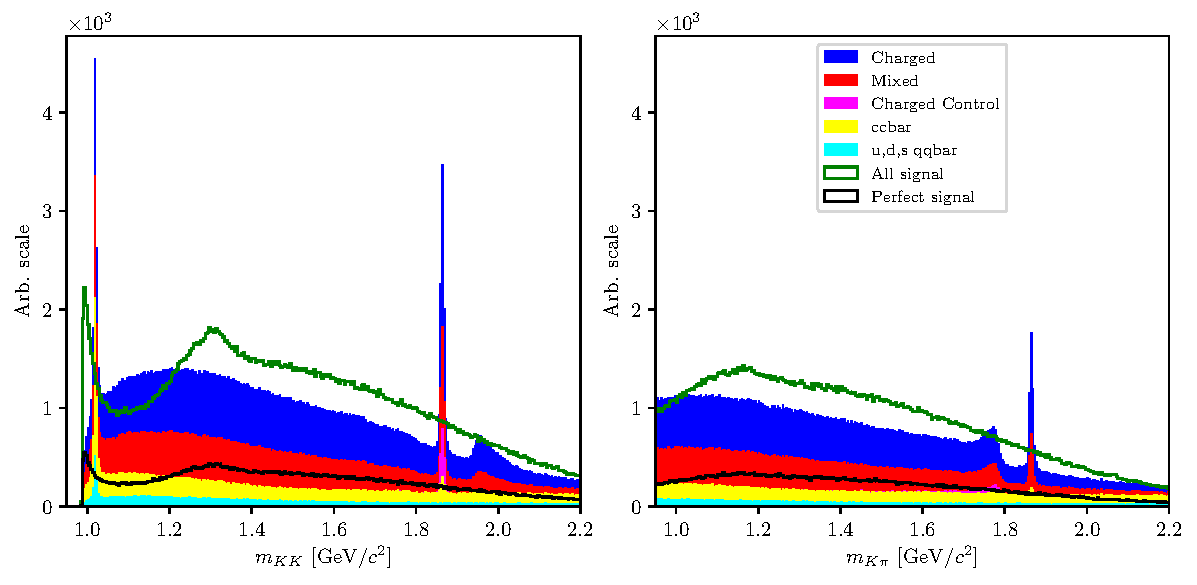
\includegraphics[width=\linewidth]{fig/res_bkg}
	\caption{Invariant mass of $KK$ candidates over a wider region (top) and for a specific region around the $\phi$ peak (bottom left), the $D^0$ peak (bottom center), and again for the $D^0$ peak, but with the $m_{K\pi}$ mass of the $KK$ candidates (bottom right). Signal (green) and perfect signal (black) are equally scaled up.}
	\label{fig:res_bkg}
\end{figure}


\section{Continuum Suppression}

Physics processes where continuum states are produced in electron and positron collisions $$e^+ e^- \to q \bar q,$$ 
with $q = u,~d,~s$ or $c$ represent an important category of backgrounds, called continuum background. In addition to kinematic constraints used before to separate $e^+ e^- \to \Upsilon(4S) \to B \bar B$ decays from $e^+ e^- \to q \bar q$, properties of the "event shape" are also used, since phase-space distributions of produced particles differ for these two processes. Continuum background events are produced back-to-back in the CMS frame, so hadrons produced in the quark fragmentation possess only a small transverse momentum compared to the initial momentum magnitude. This leads to a spatially confined, jet-like structure. On the other hand, $B$ mesons from $B \bar B$ events are produced almost at rest in the CMS frame. Their decay products form an isotropic distribution in the detector, which yields a spherical event shape.

\subsection{Characteristic Variables}
\label{ss:charvar}
Information on the phase-space distribution of produced particles can be obtained in a number of different ways. In this section different characteristic variables are presented which are used in the MVA training. They all focus on kinematic and shape differences between the two processes, which we wish to discriminate. 

%\subsubsection{$B$ meson direction}
%Two $B$ mesons, coming from a spin-1 $\Upsilon(4S)$ meson, both have 0 spin, which results in a $\sin^2\theta_B$ angular distribution of the $B$ meson direction with respect to the beam axis. On the other hand, $q \bar q$ final states are represented by two half-spin fermions, which results in two jets, following a $1+\cos^2\theta_B$ distribution. The variable $\vert \cos \theta_B \vert$ allows one to discriminate between $B$ candidates from $B \bar B$ decays and continuum background. Figure X shows the distribution of $\vert \cos \theta_B \vert$ for different $B$ meson candidates.

\subsubsection{Thrust and Related Variables}
It is possible to define a thrust axis $\vec{T}$ for a collection of $N$ momenta $p_i$ as a unit vector along which their total projection is maximal. The thrust scalar $T$ (or thrust) is a derived quantity defined as
\begin{equation}
T = \frac{\sum_{i}\vert \vec{T} \cdot \vec{p}_i\vert}{\sum_{i}\vert \vec{p}_i\vert}.
\end{equation}
In this case, a related variable is $\vert \cos\theta_T\vert$, where $\theta_T$ is the angle between the thrust axis of the particles from the $B$ meson candidate, and the thrust axis of all particles in the ROE. Since both $B$ mesons in $B \bar B$ events are produced at rest, their decay particles, and consequentially their thrust axes are isotropically distributed. On the other hand, particles in continuum events follow the direction of the jets in the event. As a consequence, both thrust axes are strongly directional and aligned in the opposite direction, which results in a large peak at $\vert \cos\theta_T\vert \approx 1$. Additionally, one can also use the variable $\vert \cos\theta_{TB}\vert $, which is the angle between the thrust axis of the $B$ candidate and the beam axis. For $B$ candidates from $B \bar B$ events, this distribution is again uniformly distributed, while for candidates from continuum events this distribution follows the distribution of the initially produced quark pairs, $1+\cos^2\theta_{T,B}$. In practice, such a distribution exhibits a drop at $\vert \cos\theta_{TB}\vert \approx 1$ due to the acceptance loss of the detector in the direction of the beam pipes. Figure \ref{fig:cosplots} shows the distributions of $\vert \cos\theta_T\vert$ (left) and $\vert \cos\theta_{T,B}\vert$ (right) for $B$ meson candidates from various sources.

\begin{figure}[H]
	\centering
	\captionsetup{width=0.8\linewidth}
	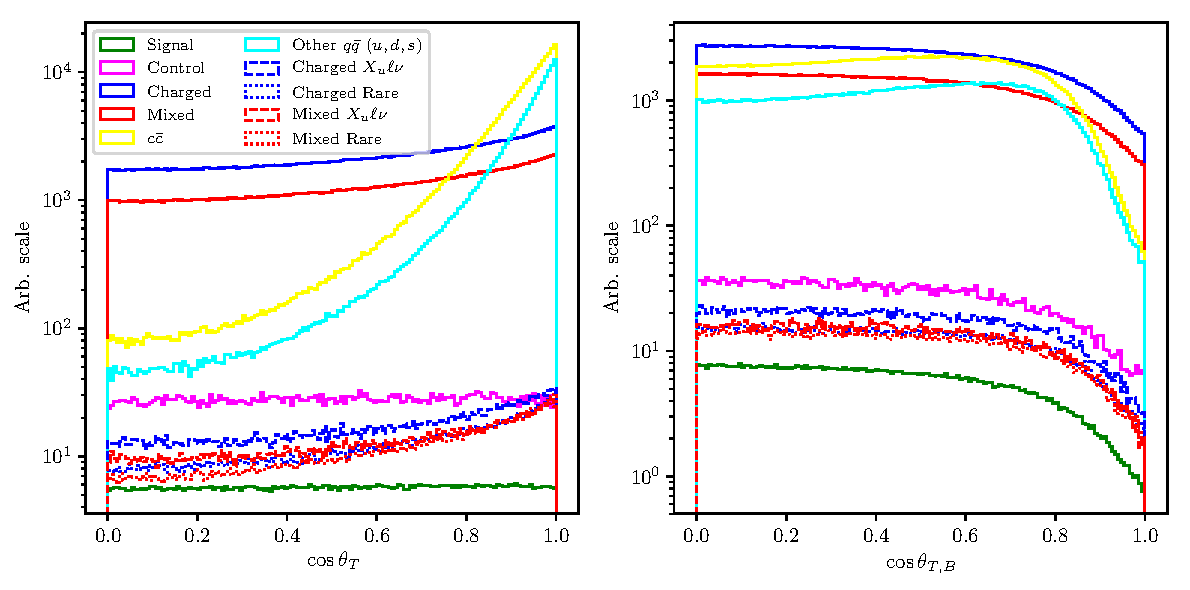
\includegraphics[width=\linewidth]{fig/cs_cosplots}
	\caption{Distributions of $\vert \cos\theta_T\vert$ (left) and $\vert \cos\theta_{T,B}\vert$ (right) for $B$ meson candidates from various sources.}
	\label{fig:cosplots}
\end{figure}

\subsubsection{CLEO Cones}
CLEO cones have been introduced by the CLEO collaboration and are an additional specific tool to provide optimal continuum background discrimination. They consist of nine variables corresponding to the momentum flow around the thrust axis of the $B$ meson candidate, binned in nine cones of $10^\circ$ around the thrust axis, as illustrated in Figure \ref{fig:ccones}. Momentum flow is defined as the scalar sum of the momenta of all charged tracks and neutral particles pointing in a specific angle interval. A Fisher discriminant is formed from the nine momentum flow variables and from $\vert \cos\theta_T\vert$ for the candidates from $q \bar q$ and $B \bar B$ events. The discriminant $\mathcal{F}$ is the linear combination of the input variables that maximizes the separation between signal and background. Additional information is provided in \cite{asner1996search}.

\begin{figure}[H]
	\centering
	\captionsetup{width=0.8\linewidth}
	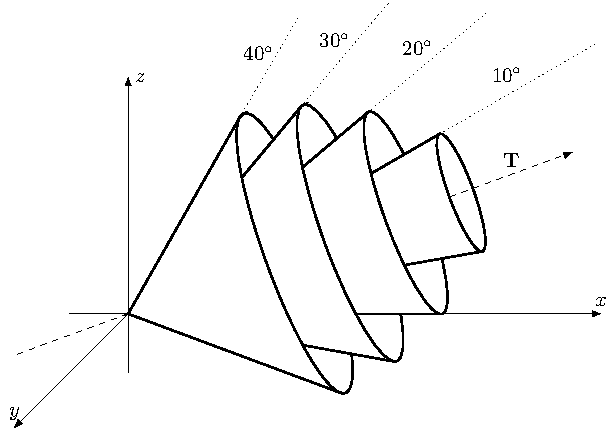
\includegraphics[scale=1]{texfig/CCones}
	\caption{Concept of CLEO cones. $\vec{T}$ denotes the thrust axis of the $B$ meson candidate in an event. Each variable corresponds to a momentum flow around the thrust axis in steps of $10^\circ$.}
	\label{fig:ccones}
\end{figure}

\subsubsection{KSFW Moments}
Fox-Wolfram moments are another useful parametrization of phase-space distribution of energy and momentum flow in an event. For a collection of $N$ momenta $p_i$, the $k$-th order normalized Fox-Wolfram moment $R_k$ is defined as
\begin{equation}
R_k = \frac{H_k}{H_0} = \frac{1}{H_0} \sum_{i,j} \vert p_i \vert \vert p_j \vert P_k(\cos \theta_{ij}),
\end{equation}
where $\theta_{ij}$ is the angle between $p_i$ and $p_j$, and $P_k$ is the $k$-th order Legendre polynomial. For events with two strongly collimated jets, $R_k$ takes values close to 0 (1) for odd (even) values of $k$, so these moments provide a convenient discrimination between $B \bar B$ and continuum events.

Belle developed a refined generation of Fox-Wolfram moments, called Kakuno-Super-Fox-Wolfram (KSFW) moments to further suppress the continuum background. They are described in detail in \cite{bevan2014physics}.

\subsubsection{\texorpdfstring{$\bm{B}$-Flavor Tagging}{B-Flavor Tagging}}
While the goal of $B$-flavor tagging is to determine the flavor of a $B$ meson, the variables used for flavor tagging also potentially contribute to background suppression. Flavor tagging relies on the fact that a large fraction of $B$ mesons decay to a final state that is flavor specific, and can  only  be   reached  either through the decay of a $b$ or a $\bar b$ quark. Because  of  the  large  number  of $B$ meson decay  channels, full reconstruction of a sufficiently large number of flavor-specific $B$ candidates  is  not  feasible. Instead  inclusive  techniques  are  employed  that  make  use  of  different
flavor-specific signatures of $B$ decays. 

The flavor tagging algorithm proceeds in two stages. In the first stage, individual flavor-specific signatures are analyzed, each of which provides a signature-specific flavor tag that by itself could be used  for  flavor  tagging.  In  the  second  stage,  the  results from the first stage signatures are combined into a final flavor  tag.  Both  stages  heavily rely on MVA  methods in order to optimally combine all available information. The final result of each stage is $qp$, a product of the flavor sign, $q$, and the probability of a correct flavor tag, $p$. Further details can be found in \cite{bevan2014physics}.

\subsubsection{ROE fit information}

Most $B$ tag mesons decay via $b \to c$ transitions with at least one additional vertex at a distance comparable to the decay length of a $B$ meson. These vertices introduce a bias in the measurement of the companion $B$ meson vertex position and degrades the vertex resolution.

The strategy to select the optimal set of tracks for the vertex determination is to first select a subset of the tracks in the ROE that satisfies requirements like a minimum number of vertex detector hits and a maximum transverse distance to the interaction region. All tracks which do not pass the selection criteria are removed. In the end, all tracks are combined in a single vertex using the interaction region as a constraint. If the goodness of the vertex fit is not good enough, the worst track is removed and the vertex refitted. This procedure is repeated until the criterion is satisfied or no tracks are left. After the vertex of the ROE has been determined, $\Delta z$ can be calculated as the distance of vertices between the signal $B$ meson candidate and the ROE in the $z$ direction.
More information is available in \cite{bevan2014physics}.

\subsection{MVA Training}
\label{ss:qqmva}
Most of the characteristic variables, described in Section \ref{ss:charvar}, were taken together in order to train a single MVA classifier for continuum suppression. All characteristic variables were checked for possible $q^2$, $M_{BC}$ or $\Delta E$ correlation. Variables with significant correlation or complex shapes in the correlation distribution were discarded from the training set, since they would have introduced unwanted dependence on the unreliable model, ISGW2, used for signal MC generation. Additionally, all of the characteristic variables in our set do not depend on the signal mode, they only differ in the kinematic and topological aspects of $B \bar B$ and continuum background events.

The training dataset consisted of $2\E5$ candidates, where $50~\%$ of the candidates are correctly reconstructed signal events, $25~\%$ are $u \bar u$, $d \bar d$ and $s \bar s$ background with expected proportions, and $25~\%$ is $c \bar c$ background. Such a composition is chosen so that there are enough signal and background samples for the MVA model training, and to avoid any of the background contributions being under-represented. Since the full Belle dataset is experiment dependent, we construct the training dataset by proportionally sampling MC events from appropriate experiments.

The training variable set consisted of
\begin{itemize}
	\item $B$ meson direction and thrust related variables
	\begin{itemize}
		\item magnitude of thrust axes of the $B$ and $ROE$ candidates,
		\item cosine of the angle between the thrust axis of the $B$ candidate and thrust axis of the ROE candidate,
		\item cosine of the angle between the thrust axis of the $B$ candidate and the beam direction,
		\item reduced Fox-Wolfram moment $R_2 $,
	\end{itemize}
	\item all $9$ CLEO Cones
	\item KSFW Moments
	\begin{itemize}
		\item $R^{so}_{01}$, $R^{so}_{02}$, $R^{so}_{03}$, $R^{so}_{04}$,
		\item $R^{so}_{10}$, $R^{so}_{12}$, $R^{so}_{14}$,
		\item $R^{so}_{20}$, $R^{so}_{22}$, $R^{so}_{24}$,
		\item $R^{oo}_{0}$, $R^{oo}_{1}$, $R^{oo}_{2}$, $R^{oo}_{3}$, $R^{oo}_{4}$,
	\end{itemize}
	\item $B$-flavor tagging variables
	\begin{itemize}
		\item $qp$ of $e,~\mu,~\ell$,
		\item $qp$ of intermediate $e,~\mu,~\ell$,
		\item $qp$ of $K$, $K/\pi$, slow pion, fast hadron,
		\item $qp$ of maximum $P^*$, $\Lambda$, fast-slow-correlated (FSC),
	\end{itemize}
	\item Other
	\begin{itemize}
		\item $\Delta z$.
	\end{itemize}
\end{itemize}

Figure \ref{fig:cs_mva} shows the classifier output for various types of background, all in expected MC proportions. $B$ meson candidates from continuum background are dominant at lower values, while candidates from $B \bar B$ events populate the region with higher values.

\begin{figure}[H]
	\centering
	\captionsetup{width=0.8\linewidth}
	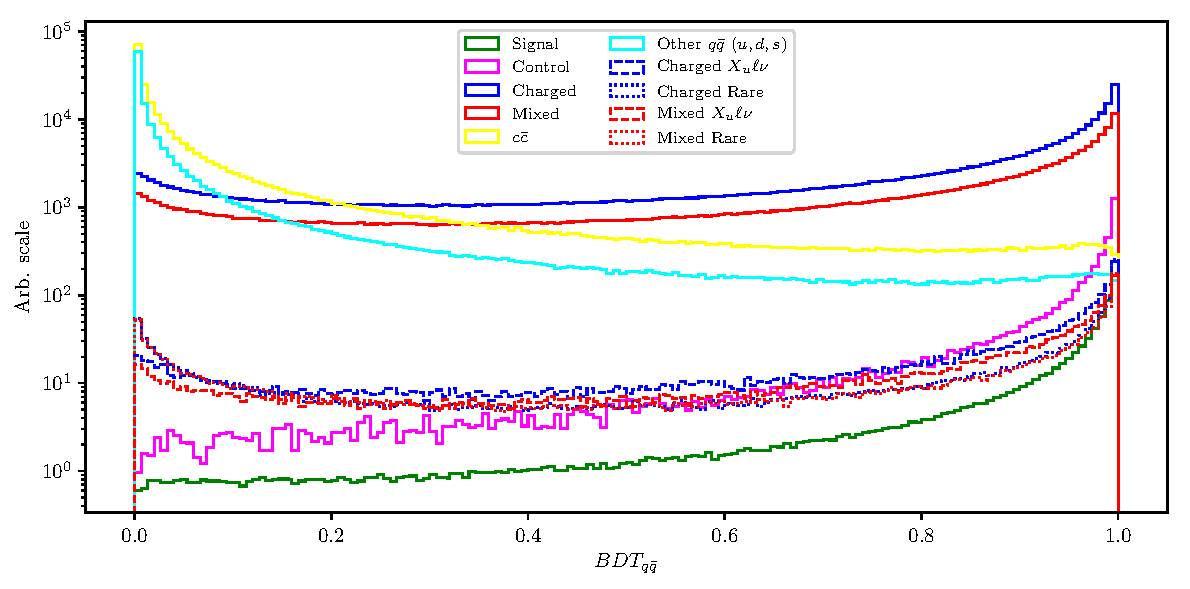
\includegraphics[width=\linewidth]{fig/cs_BDT}
	\caption{Continuum suppression classifier output for signal and various types of background. $B$ candidates from continuum events dominate the lower region, while candidates from $B\bar B$ dominate in the upper region of the classifier output.}
	\label{fig:cs_mva}
\end{figure}

\section{\texorpdfstring{$B\bar B$}{BB-bar} Suppression}

After separating continuum background from $B \bar B$ events, the next step is to train an MVA classifier to recognize our signal candidates among the candidates from other $B \bar B$ background. $B \bar B$ events consists of
\begin{itemize}
	\item $b \to c \ell \nu$ background,
	\item $b \to u \ell \nu$ background,
	\item Other rare decays (radiative, penguin, rare 2- and 3-body decays, \dots).
\end{itemize}

Similarly, the training dataset for this classifier consisted of $2\E5$ candidates, where $50~\%$ of the candidates are correctly reconstructed signal events. The remaining part of the training dataset consists of all background, not including the control sample, because we are not interested in suppressing it directly. The background part of the dataset consists of $75~\%$  generically decaying charged and neutral $B \bar B$ events in equal proportions, whereas the remaining $25~\%$ is equally populated with charged and neutral $B \bar B$ events from $b \to u \ell \nu$ and other rare decays. The training dataset was proportionally sampled in the same manner as described in Section \ref{ss:qqmva}.

In order to separate this kind of background, we must be careful not to introduce correlations with the fit variables ($\Delta E$, $M_{BC}$) or any kind of model dependence (correlation with $q^2$). This means that we can not use any information of the decay particles or the candidate, which is of kinematic nature, such as decay particles momenta, decay angles or similar.

The training variable set consisted of
\begin{itemize}
	\item vertex fit probability of $P(\chi^2,DOF)$ of the signal $B$ meson candidate
	\item vertex fit probability of $P(\chi^2,DOF)$ of the ROE side,
	\item $\cos\theta_{BY}$ from Eq. (\ref{eq:cosby}),
	\item $\cos$ of the angle between the momentum vector and vector joining the IP and the production vertex of the $KK\ell$ candidate,
	\item $B$-flavor tagging variables for the two signal-side kaons,
	\item numbers of kaons, tracks and distant tracks in ROE,
	\item $\theta$ angle of the ROE momentum in CMS frame,
	\item $\xi_Z$ from \cite{PhysRevD.83.032007}
	\item $\Delta z$,
	\item $m_{miss}^2$ from Eq. (\ref{eq:m2def}),
	\item $m_{miss}^2$ for partial reconstruction of $B^0 \to D^{*-} \ell \nu$,
\end{itemize}
where distant tracks are all tracks in ROE which satisfy the condition of $\vert d_0 \vert  > 10.0\e{cm}$ or $\vert z_0 \vert > 20.0\e{cm}$. The last entry is a veto variable where we partially reconstruct the $D^*$ candidate four-momentum via a linear combination of the $\pi^\pm_s$ four-momentum in the $D^* \to D \pi_s^\pm$ decay. It contributes to discarding the $B^0 \to D^{*-} \ell^+ \nu$ decay, where $D^{*-}$ further decays to $D^{*-} \to \bar D {}^0 \pi^-_s$. Figure \ref{fig:vetoplot} shows the veto variable with a partial reconstruction of a charged $\pi_s^\pm$.

\begin{figure}[H]
	\centering
	\captionsetup{width=0.8\linewidth}
	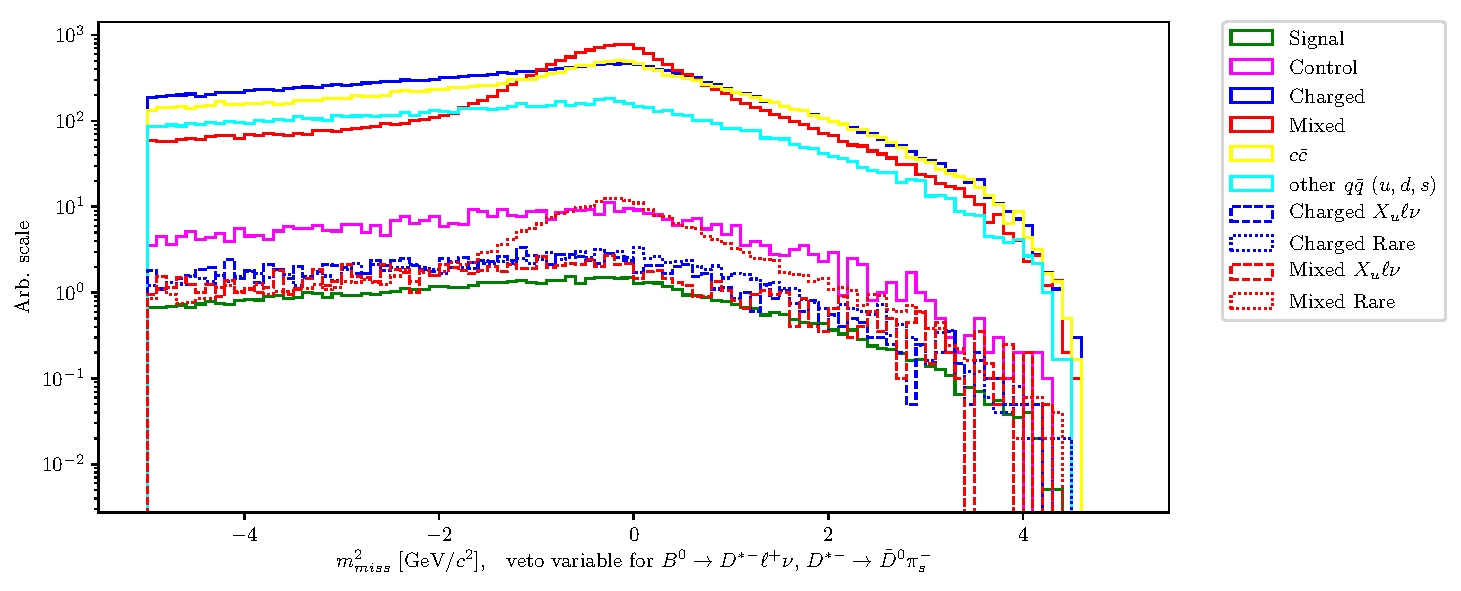
\includegraphics[width=\linewidth]{fig/bb_partial_veto}
	\caption{Distribution of $m_{miss}^2$ for partially reconstructed $B^0 \to D^{*-} \ell^+ \nu$ decays.}
	\label{fig:vetoplot}
\end{figure}

When the training is finished and the hyper-parameters of the classifier are optimized, the classifier output, as shown in Figure \ref{fig:bbmva} (left), can be used for background suppression. $B$ meson candidates from $B \bar B$ background are dominant at lower values, while candidates from $B \bar B$ events populate the region with higher values. Since the differences between signal and background $B \bar B$ events are smaller than $B \bar B$ and $q \bar q$ events, the resulting classifier has a smaller separation power than the one described in the previous section.

\subsection{Boosting to Uniformity}
The selection approach with standard classifiers is optimal for counting experiments, as it, by construction, produces the optimal selection for observing an excess of signal over background events. Today's BDT algorithms, which work in this way, produce non-uniform selection efficiencies and may, as a consequence, shape background distributions to look like signal. In order to minimize such behavior, it is possible to discard variables, which are correlated with the variable of interest (in our case \vars), from the training set. This, however, decreases the classifiers discriminating power. Another approach is to use a novel boosting method, uBoost, which is trained to optimize an integrated $FOM$ under the constraint that the BDT selection efficiency for the desired class must be uniform. The uBoost algorithm balances the biases to produce the optimal uniform selection \cite{stevens2013uboost}.

The training set used is the same as described at the beginning of this chapter, along with the same set of training variables. It will be seen later that the standard $BDT$ classifier shapes the background to look like signal mostly in the $M_{BC}$ distribution, therefore we train the $uBDT$ classifier with a uniformity constraint on the $M_{BC}$ variable of the background candidates. The resulting classifier output is shown in Figure \ref{fig:bbmva} (right). For this classifier, the separation power between signal and background seems worse, however, the shapes of backgrounds differ significantly, which greatly affects the performance of signal extraction.

\begin{figure}[H]
	\centering
	\captionsetup{width=0.8\linewidth}
	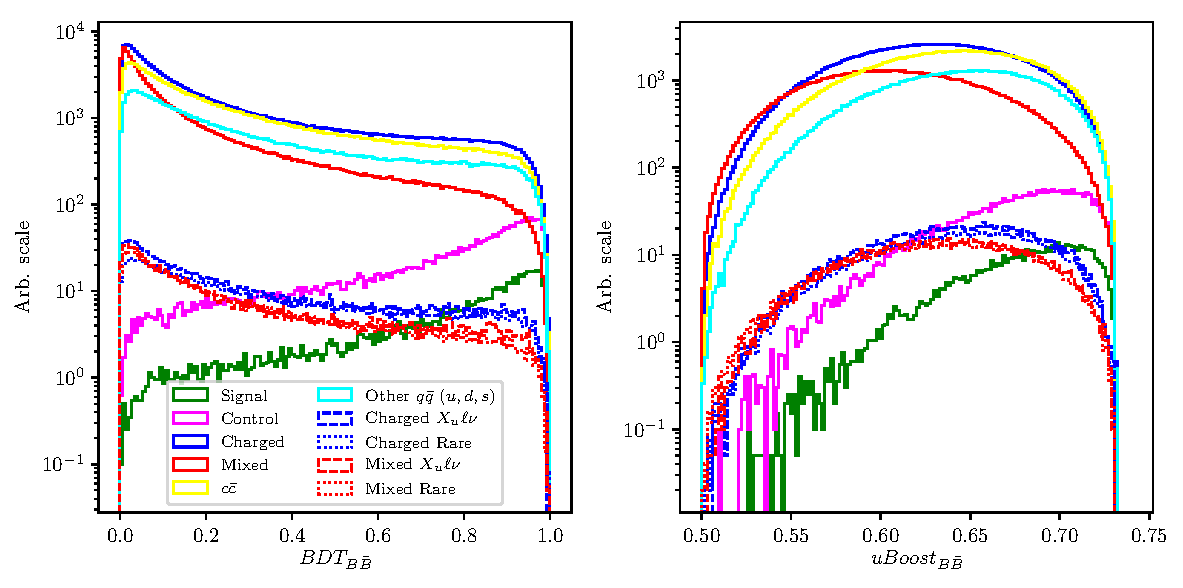
\includegraphics[width=\linewidth]{fig/bb_BDT}
	\caption{$B\bar B$ suppression classifier output for signal and various types of background for the standard $BDT$ classifier (left) and the $uBDT$ classifier (right). $B$ candidates from $B\bar B$ background events dominate the lower region, while signal and control candidates dominate in the upper region of the classifier output.}
	\label{fig:bbmva}
\end{figure}

\section{Selection Optimization}\label{sec:selection-optimization}

Instead of two separate $q \bar q$ and $B \bar B$ $FOM$ optimizations, it is more efficient to do a simultaneous 2D $FOM$ optimization, since the two classifiers are not completely uncorrelated. In the same manner as before, $FOM$ is optimized for perfectly reconstructed signal candidates in the signal window, after the pre-selection, signal categorization, and after discarding the background resonances and the control decay. The $FOM$ plot with the optimal point for both $B \bar B$ MVA classifiers is shown in Figure \ref{fig:mvafom}.

\begin{figure}[H]
	\centering
	\captionsetup{width=0.8\linewidth}
	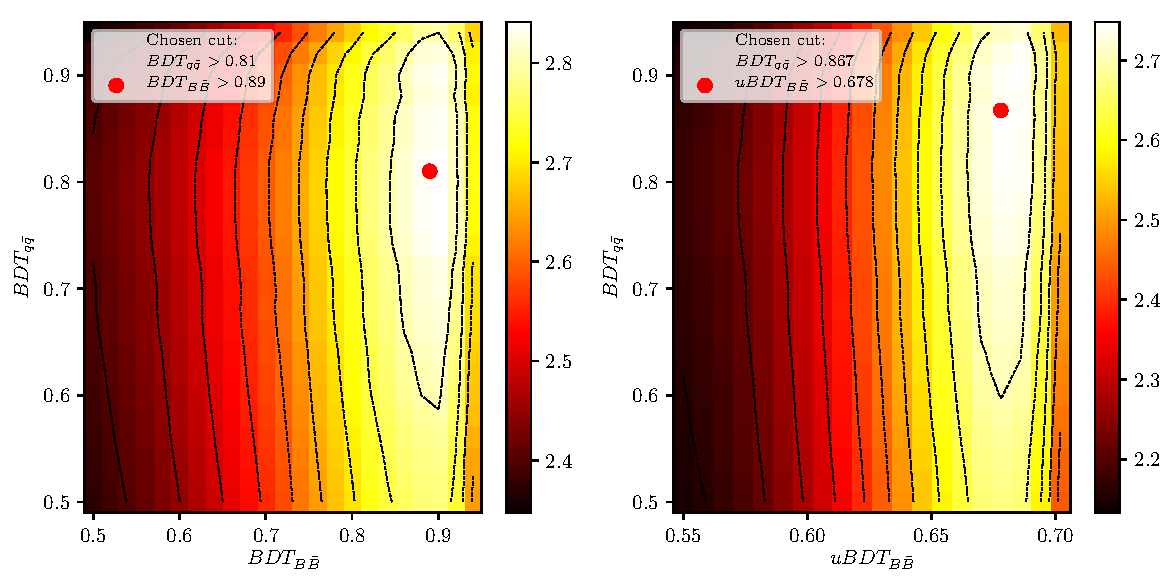
\includegraphics[width=\linewidth]{fig/mva_fom}
	\caption{2D $FOM$ optimization of continuum suppression classifier and the standard $BDT$ (left) and $uBDT$ (right) $B\bar B$ suppression classifier.}
	\label{fig:mvafom}
\end{figure}

We can compare signal and major background distributions of \vars~after the 2D $FOM$ optimization for both classifiers. Figure \ref{fig:opt01c} shows the arbitrary (left) and normalized scale (right) for $\Delta E$ (top) and $M_{BC}$ (bottom) for the final sample optimized with the standard $BDT$ classifier, while Figure \ref{fig:opt1dc} shows similarly for the final sample optimized with $uBDT$ classifier. We can see that there is considerably more background in the latter case, however, also shapes of background and signal distributions differ greatly, meaning there is less room for correlation. The biggest change seems to be in the shape of the $M_{BC}$ distribution, where the background component is much more signal like in the final sample optimized with the standard $BDT$ classifier than in the other case.  Additionally, the shapes are more easily constrained in the latter case, since they are present in regions where no signal is expected. The total numbers of expected signal candidates and the signal-to-noise ratios for both classifiers are:
\begin{itemize}
	\item Standard $BDT$: $N_{sig} = 176,\quad N_{sig}/N_{bkg} = 4.83~\%$,
	\item $uBDT$: $N_{sig} = 264,\quad N_{sig}/N_{bkg} = 1.33~\%$.
\end{itemize}
Due to the large difference in \vars~shape, we will continue the analysis with the $uBDT$ classifier, although the comparison between both methods will be shown for the final fit result in the next chapter.

\begin{figure}[H]
	\centering
	\captionsetup{width=0.8\linewidth}
	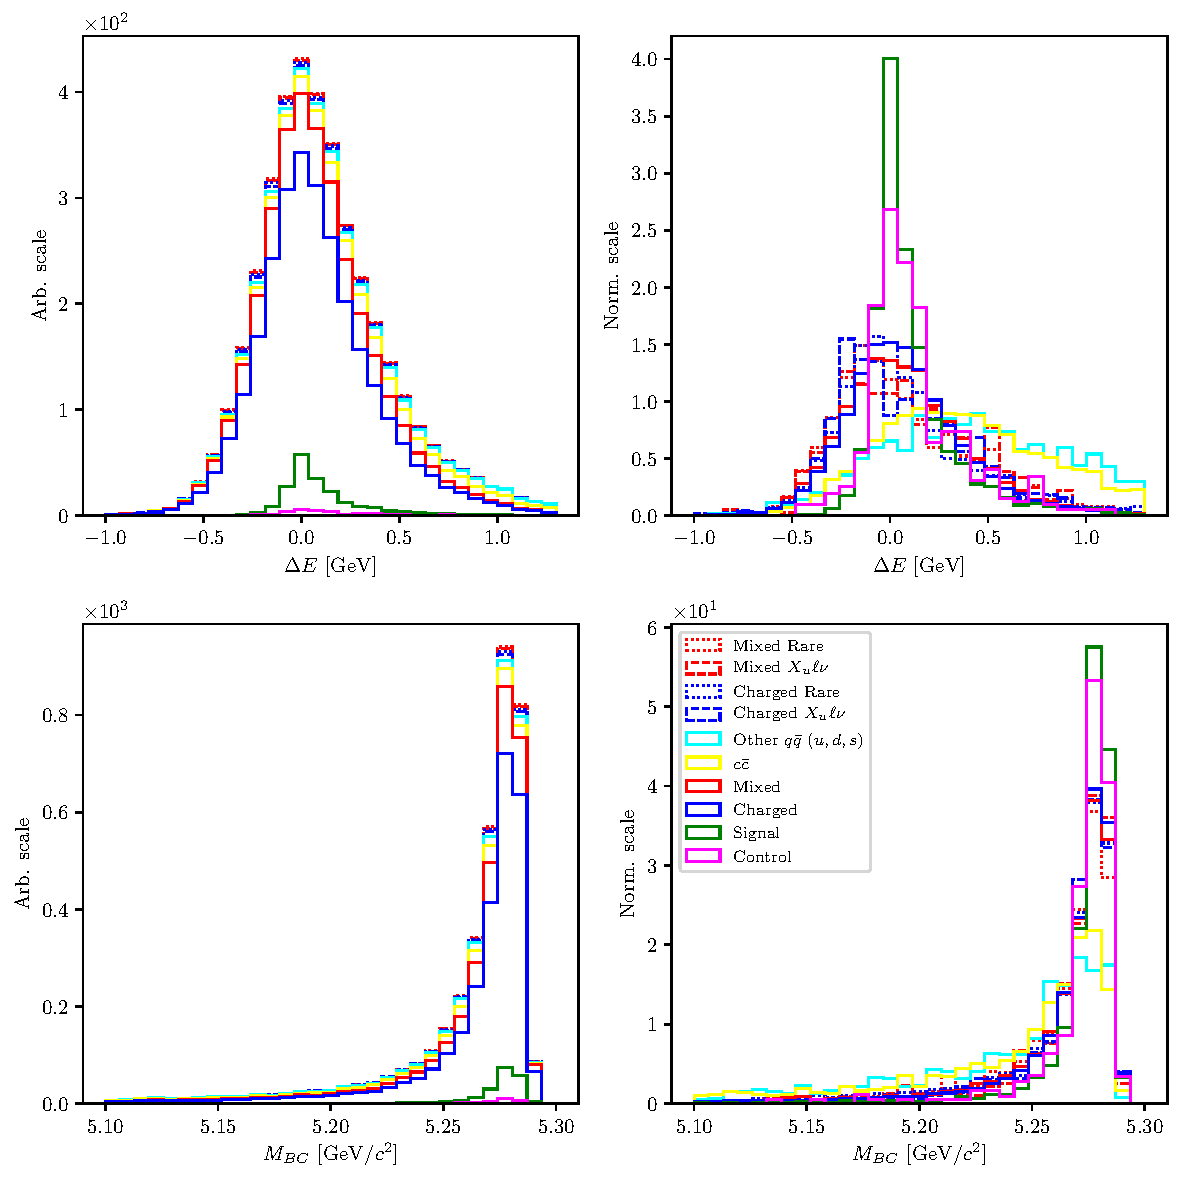
\includegraphics[width=\linewidth]{fig/opt_BB}
	\caption{Arbitrary (left) and normalized scale (right) for $\Delta E$ (top) and $M_{BC}$ (bottom) for the final sample optimized with the standard $BDT$ classifier.}
	\label{fig:opt01c}
\end{figure} 

\begin{figure}[H]
	\centering
	\captionsetup{width=0.8\linewidth}
	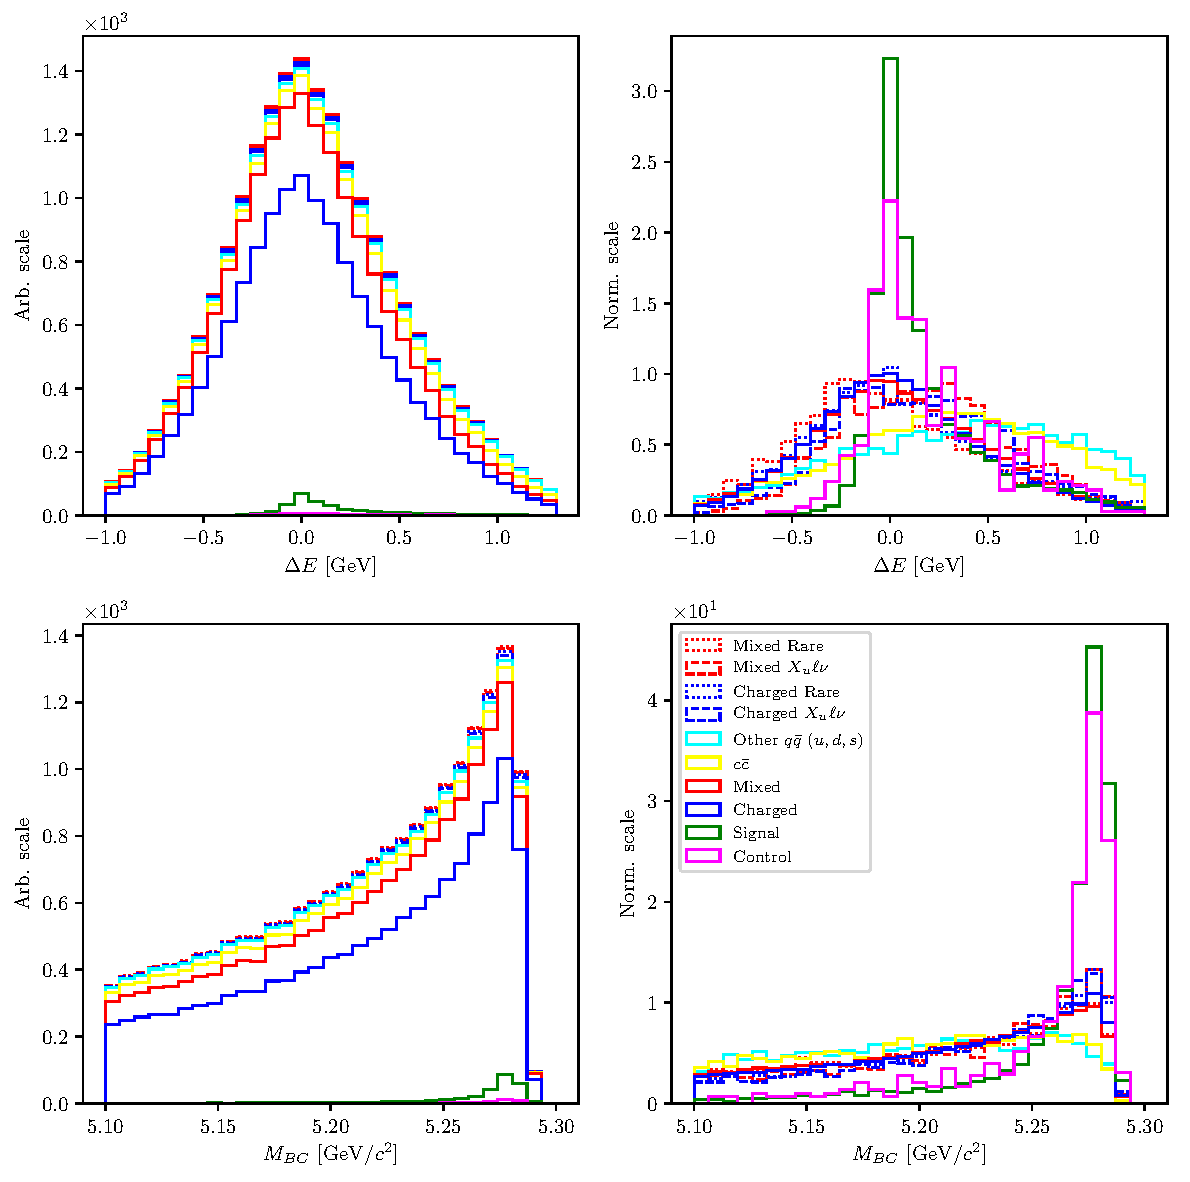
\includegraphics[width=\linewidth]{fig/opt_uBB}
	\caption{Arbitrary (left) and normalized scale (right) for $\Delta E$ (top) and $M_{BC}$ (bottom) for the final sample optimized with the $uBDT$ classifier for $B \bar B$ suppression.}
	\label{fig:opt1dc}
\end{figure} 

\subsection{\texorpdfstring{$B \bar B$}{BB-bar} Background Composition and Lepton Veto}

The majority of background candidates after the final selection is represented by candidates from $B \bar B$ events. In order to suppress this background even further, we need to take a look at its structure and recognize various contributions to this part of the background. Figure \ref{fig:sig_bkg_all_before} shows \vars, and $m_{KK}$ for the most significant contributions in the signal region. While most of the candidates come from events where all reconstructed charged particles in the signal decay do not come from a single $B$ meson, but both of them, these candidates are not so problematic. Their distribution is rather smooth and frequent in regions where we expect no signal. On the other hand, there are also contributions from some specific $B$ meson decays which produce more signal-like distributions. We will denote the first kind of background as $\Upsilon(4S)$-matched and the second kind as the $B$-matched $B \bar B$ background. Fortunately, these decays are well known and well measured, so their yields can be constrained. Especially problematic is the double semileptonic decay $B \to \bar D {}^{(*)} \ell^+ \nu,~D^+ \to \bar K^- \ell^+ \nu$, where the secondary lepton is misidentified as a kaon. Even though the decay has two neutrinos, these events survive the $m_{miss}^2$ selection and produce peaks at the same positions as the signal distributions, while exhibiting only a slightly worse resolution. 

\begin{figure}[H]
	\centering
	\captionsetup{width=0.8\linewidth}
	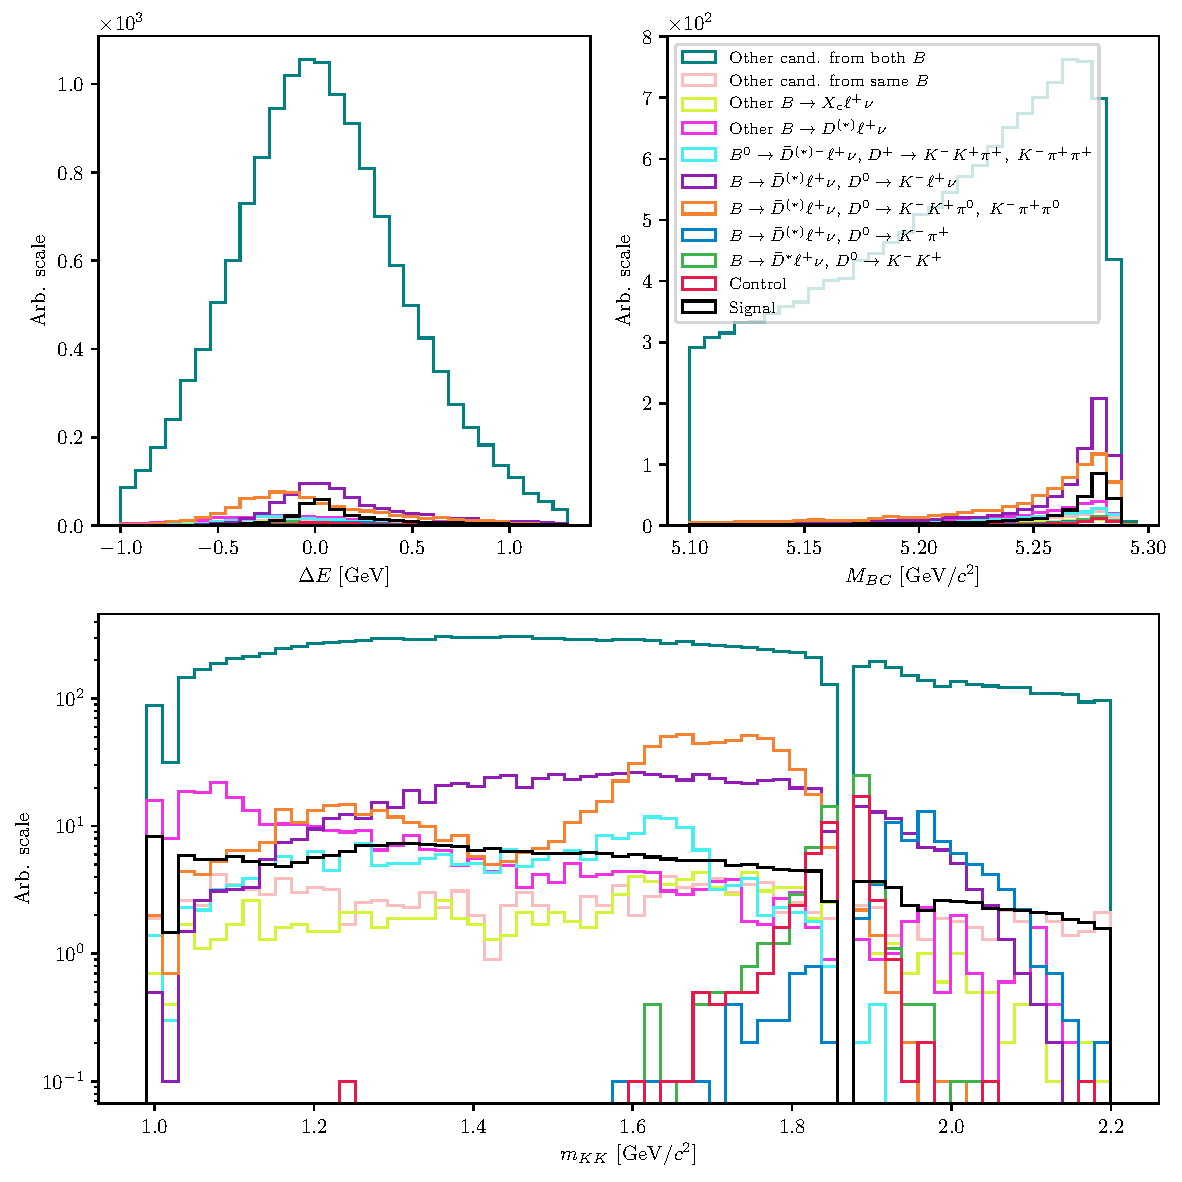
\includegraphics[width=\linewidth]{fig/sig_BKG_composition_all_before.pdf}
	\caption{$\Delta E$ (left), $M_{BC}$ (right) and $m_{KK}$ (bottom) for major contributions to the $B \bar B$ background in the signal region. $\Upsilon(4S)$-matched backgrounds represents the majority, but have a smooth and wide distribution, distinguishable from signal. $B$-matched contributions show a peak in $M_{BC}$ and sometimes in $\Delta E$, but can be constrained using existing measurements.}
	\label{fig:sig_bkg_all_before}
\end{figure} 

In order to suppress the latter source of background, a lepton veto can be applied to both kaons, requiring that neither of the kaons should exhibit lepton-like properties. On the candidates passing the final selection, we optimize the $eID$ and $\mu ID$ PID cuts, where $S$ and $B$ in Eq. \ref{eq:fom} are represented by perfect signal candidates and by background candidates, respectively. Background in this case is represented by events in which a lepton has been misidentified as a kaon. 2D $FOM$ plots for both kaons are shown in Figure \ref{fig:lepVeto}, where $K_0$ denotes same-sign, and $K_1$ the opposite-sign kaon, with respect to the $B$ meson which they are part of. It can be seen that in the majority of cases an electron is misidentified as $K_1$. With the optimal selection 
\begin{itemize}
	\item $K_0:~eID < 0.8,$
	\item $K_1:~eID < 0.1,~\mu ID < 0.8,$
\end{itemize}
we reject $77.5\%$ of candidates from the double semileptonic decays, while efficiency loss of signal and other types of $B \bar B$ background is about $5-6\%$. The $B \bar B$ background after the lepton veto is shown in Figure \ref{fig:sig_bkg_all_after} for the signal region, and in Figure \ref{fig:cs_bkg_after} for the control region.

\begin{figure}[H]
	\centering
	\captionsetup{width=0.8\linewidth}
	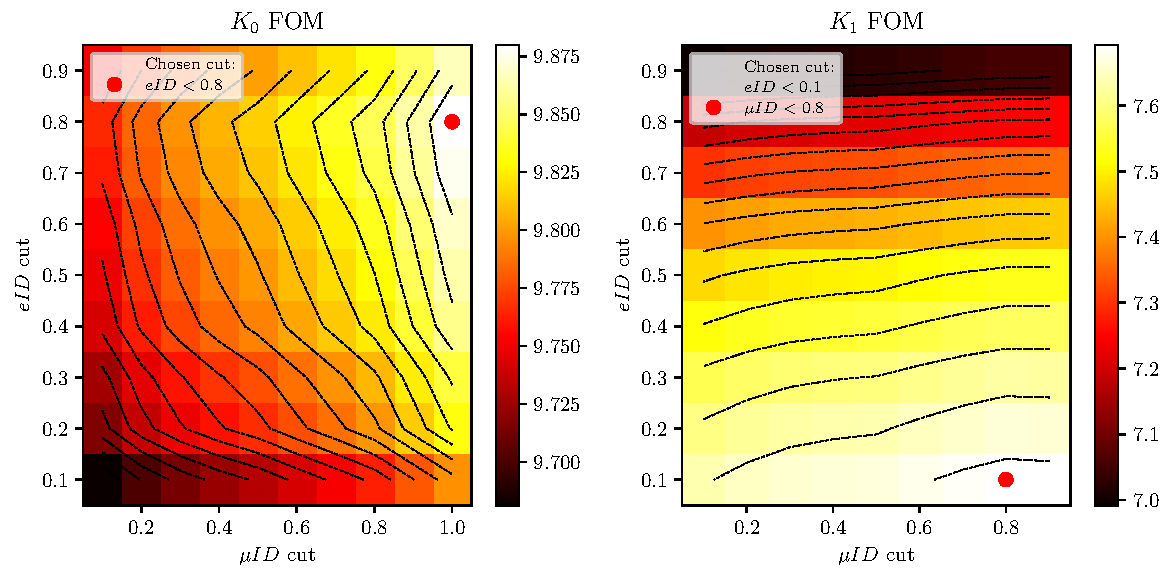
\includegraphics[width=\linewidth]{fig/lepVeto}
	\caption{2D $FOM$ for optimal $eID$ and $\mu ID$ selection on same-sign (left) and opposite-sign (right) kaons with respect to the $B$ meson charge. For double semileptonic background component, in most cases an electron is missidentified as the opposite-sign kaon in the reconstruction chain.}
	\label{fig:lepVeto}
\end{figure} 

\begin{figure}[H]
	\centering
	\captionsetup{width=0.8\linewidth}
	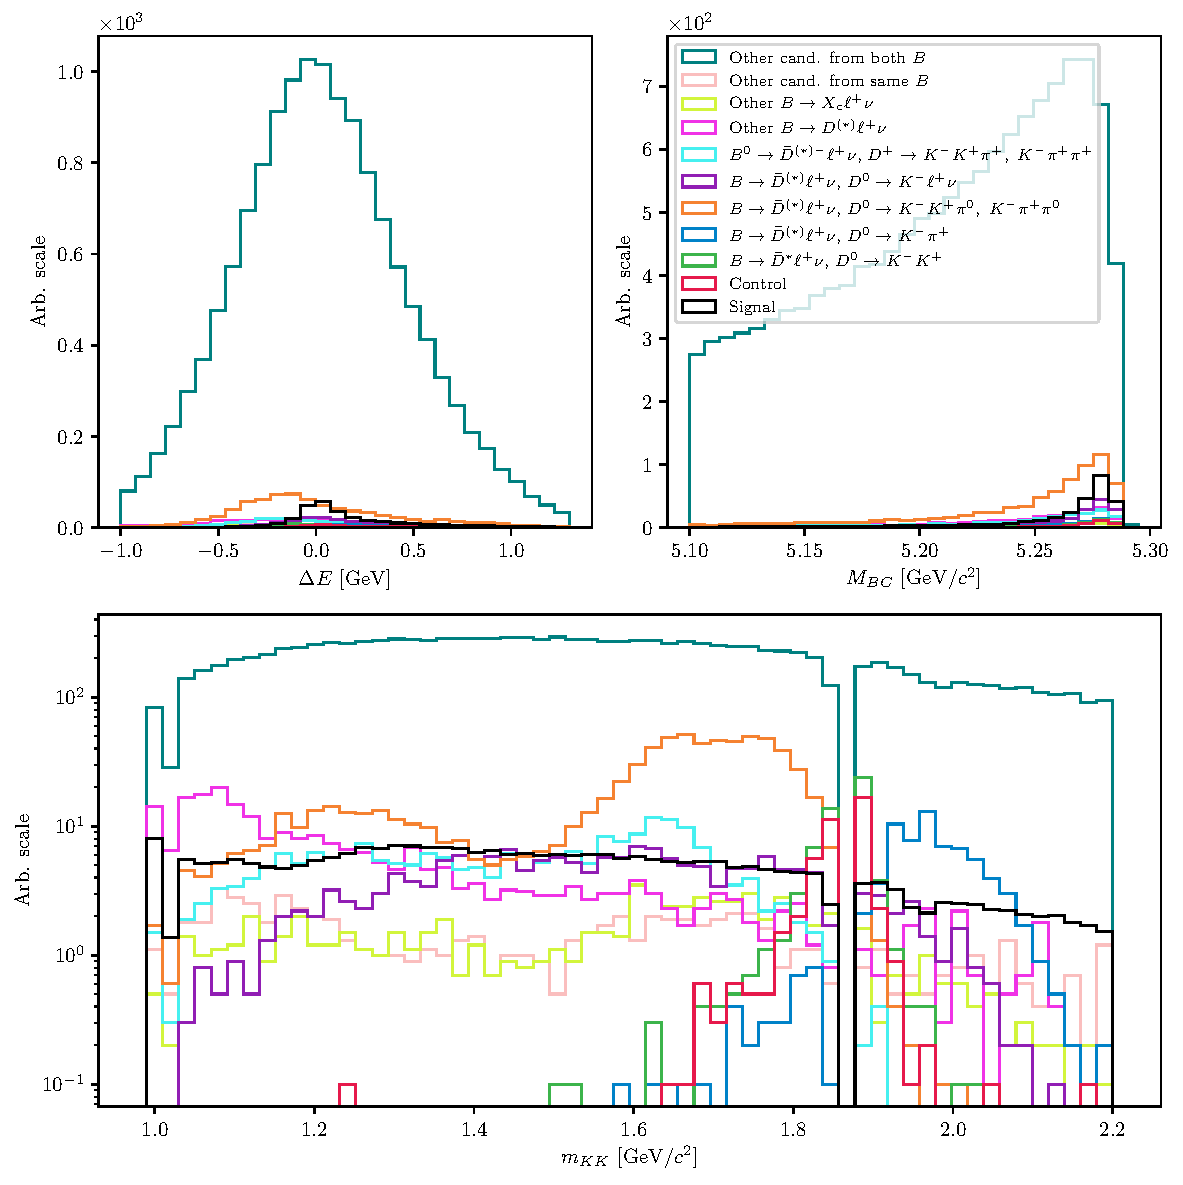
\includegraphics[width=\linewidth]{fig/sig_BKG_composition_all_after}
	\caption{$\Delta E$ (left), $M_{BC}$ (right) and $m_{KK}$ (bottom) for major contributions to the $B \bar B$ background in the signal region after the lepton veto. The double semileptonic background component is suppressed by a factor of $4-5$.}
	\label{fig:sig_bkg_all_after}
\end{figure} 

\begin{figure}[H]
	\centering
	\captionsetup{width=0.8\linewidth}
	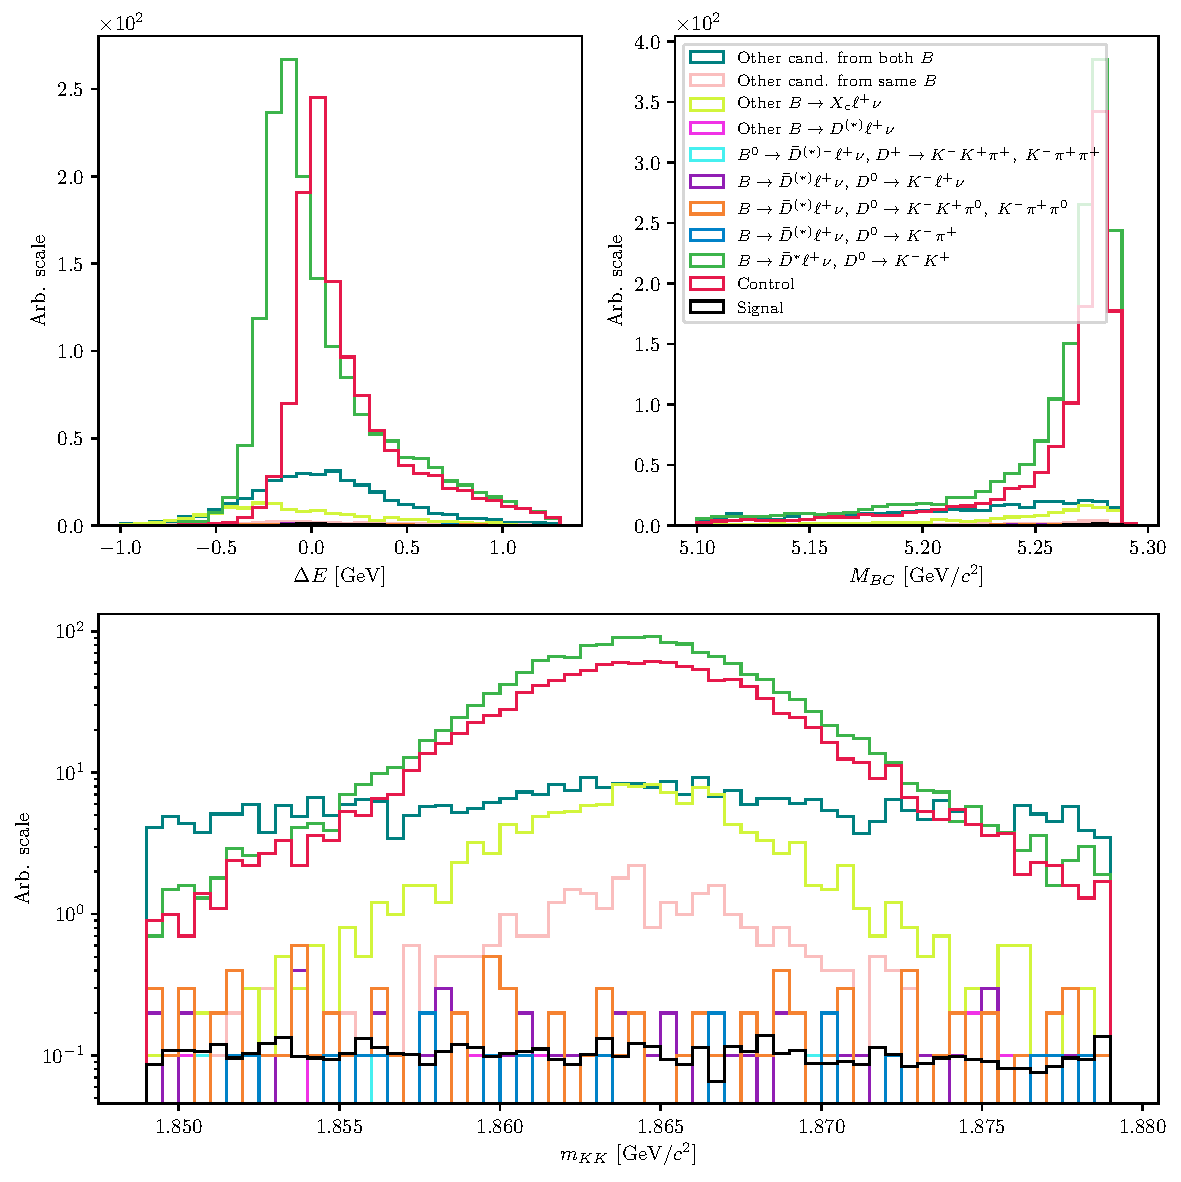
\includegraphics[width=\linewidth]{fig/cs_BKG_composition_after}
	\caption{$\Delta E$ (left), $M_{BC}$ (right) and $m_{KK}$ (bottom) for major contributions to the $B \bar B$ background in the control region after the lepton veto. The major component in this case are other $B \to D^* \ell+ \nu,~D \to K^+K^-$ decays, besides the control decay.}
	\label{fig:cs_bkg_after}
\end{figure} 

\section{Data and MC Agreement}

With the final selection in place, we can check the data and MC agreement by checking the control decay region in on- and off- resonance data. Off-resonance samples provide the ability to check the agreement of the $q\bar q$ background component, while on-resonance samples can be used to check the validity of the control MC sample and, consequently, the signal MC sample.

\subsection{Off-resonance Data}

The off-resonance data were collected at $60\e{MeV}$ below the $\Upsilon(4S)$ resonance peak energy in order to determine the continuum background. It therefore offers a direct view of the $q\bar q$ background data sample, which we can compare to the off-resonance MC sample. Figure \ref{fig:offres_control} shows $\Delta E$, $M_{BC}$ and the $q \bar q$ classifier output, $BDT_{q\bar q}$, for off-resonance data and stacked MC in the control region, before the MVA selection, where the MC sample was scaled down by a factor of $6$, due to 6 streams of MC. These figures do not show a fit to the data, but merely an overlay of data and stacked MC distributions, and show good data and MC agreement of the off-resonance sample already before the fit. More importantly than the normalization, the shape of data and MC also seems to match, so further corrections of \vars~on MC are not necessary. This is also demonstrated by the flatness of the ratio of \vars~distributions, shown in the same Figure. There seems to be a difference in the classifier performance for the continuum background suppression on data and MC in the lower region of $BDT_{q \bar q}$, where classifier efficiency on MC is overestimated. However, after the selection on classifier output, these differences are negligible, since a relatively small amount of continuum background passes the selection.
\begin{figure}[H]
	\centering
	\captionsetup{width=0.8\linewidth}
	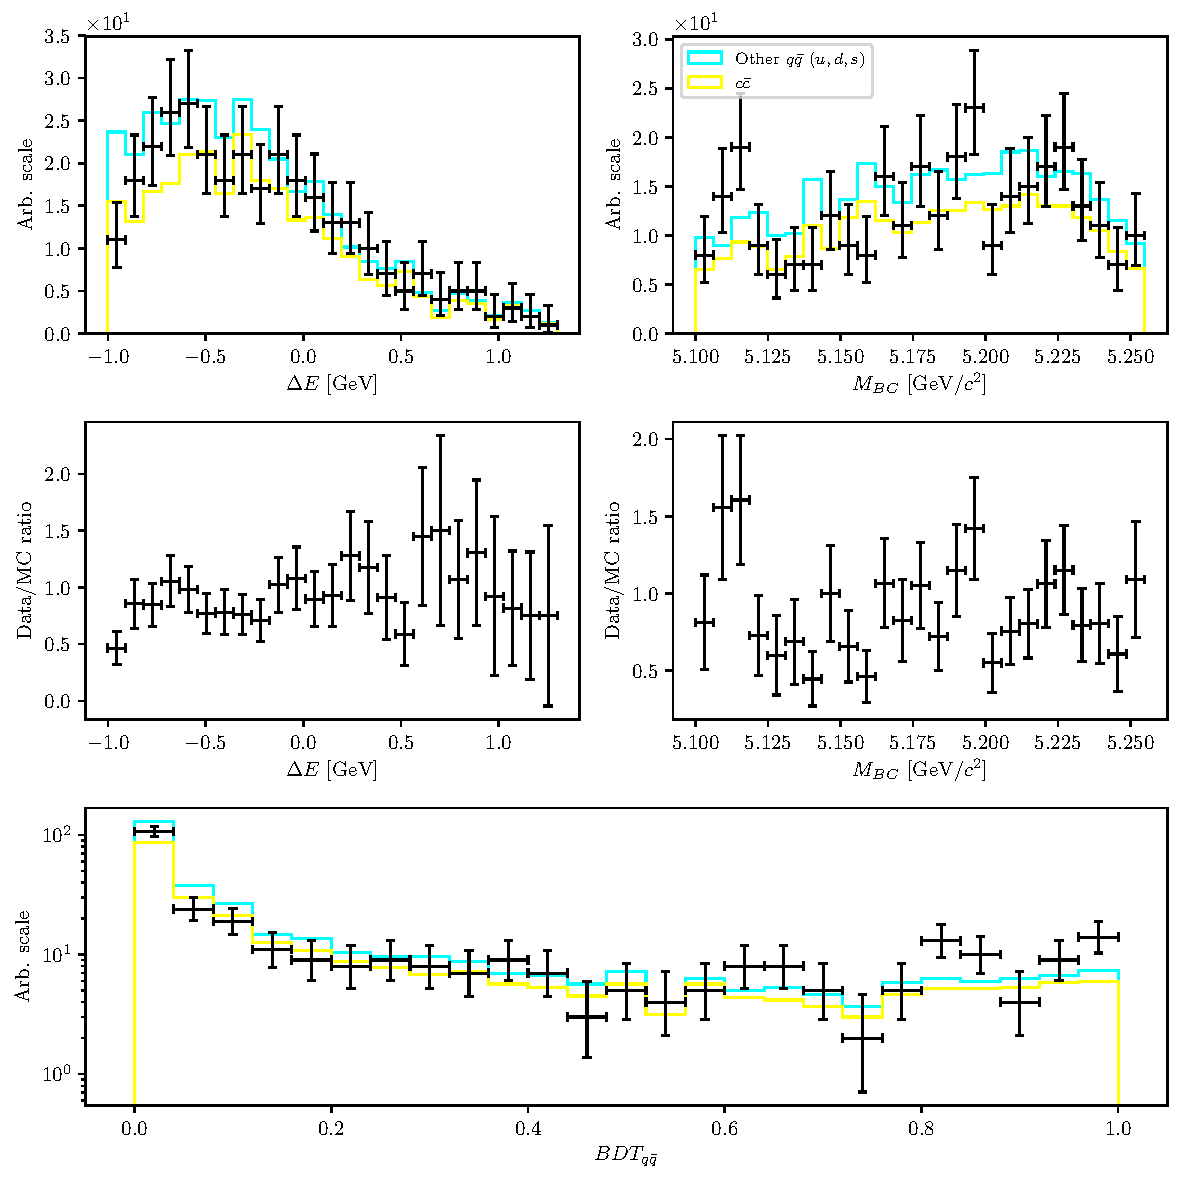
\includegraphics[width=\linewidth]{fig/offres_control}
	\caption{$\Delta E$ (left), $M_{BC}$ (right) and the $q \bar q$ classifier output (bottom), for off-resonance data and MC in the control region prior to any MVA selection.}
	\label{fig:offres_control}
\end{figure}

\subsection{On-resonance Data}

We can repeat the check on on-resonance data. Figure \ref{fig:onres_control} shows $\Delta E$, $M_{BC}$, $BDT_{q \bar q}$ and $uBDT_{B \bar B}$, where one can see inconsistencies between data and stacked MC on the lower parts of all $BDT$ spectra. These figures again do not show the fit, but merely an overlay of data to the stacked MC distributions. On the other hand, data and MC seem to agree well in the upper parts of the spectra. Overall, data and MC seem to agree well after the pre-selection and without any corrections. This means that the modeling of the MC sample is precise and that the MVA selection does not introduce any additional differences between data and MC for the control sample, and therefore the signal sample.
\begin{figure}[H]
	\centering
	\captionsetup{width=0.8\linewidth}
	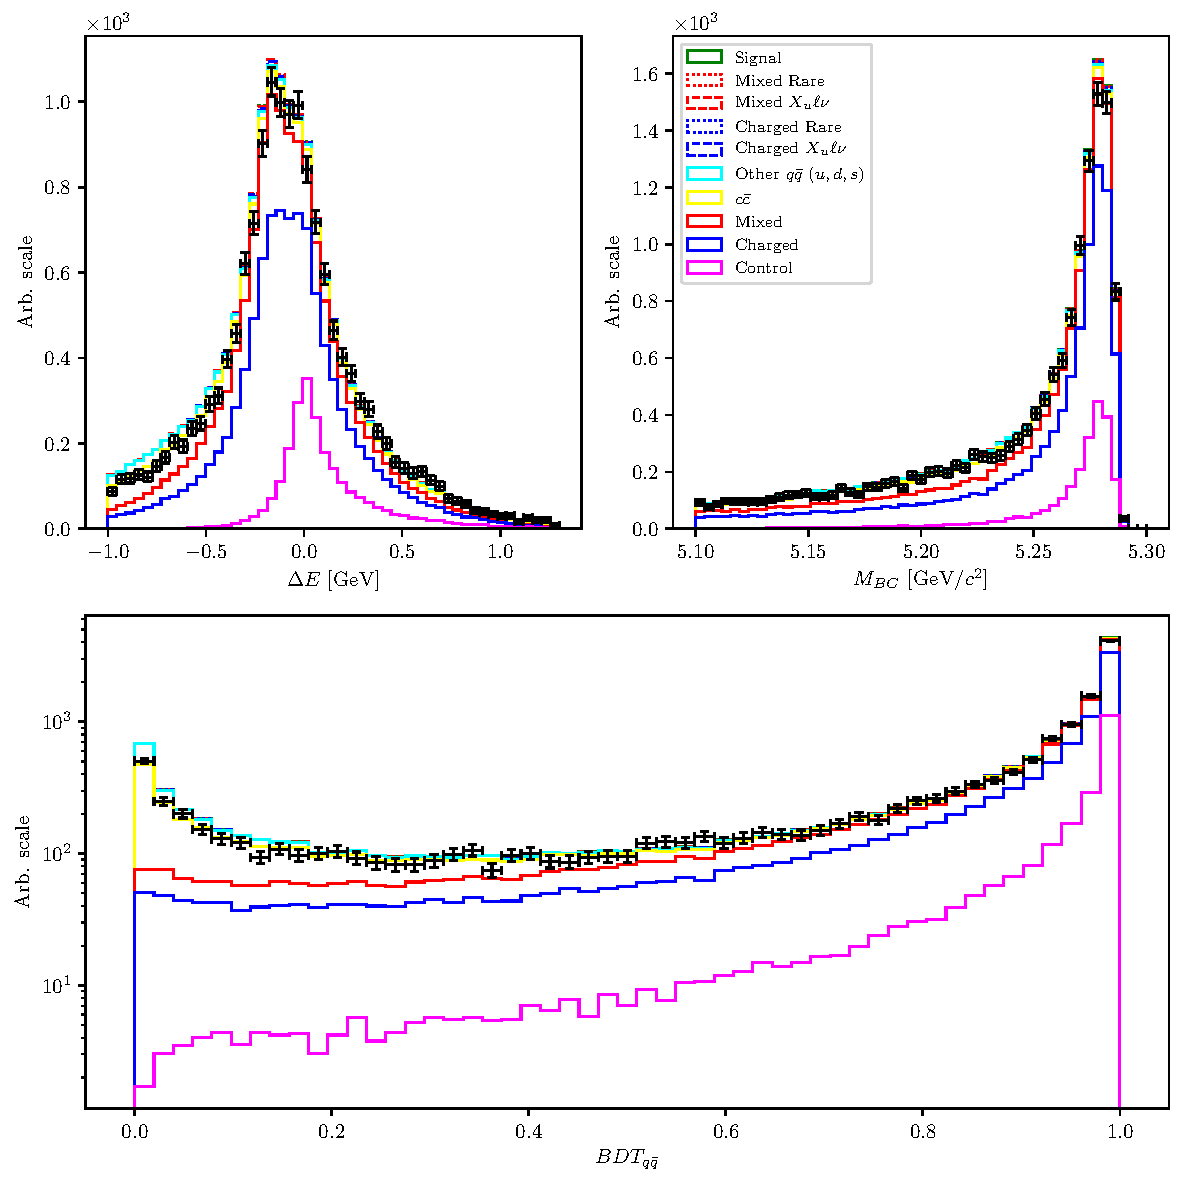
\includegraphics[width=\linewidth]{fig/onres_control}
	\caption{$\Delta E$ (top left), $M_{BC}$ (top right), the $q \bar q$- (bottom left) and the $B \bar B$ classifier output (bottom right), for on-resonance data and MC in the control region prior to the MVA selection.}
	\label{fig:onres_control}
\end{figure}